% This is "sig-alternate.tex" V2.0 May 2012
% This file should be compiled with V2.5 of "sig-alternate.cls" May 2012
%
% This example file demonstrates the use of the 'sig-alternate.cls'
% V2.5 LaTeX2e document class file. It is for those submitting
% articles to ACM Conference Proceedings WHO DO NOT WISH TO
% STRICTLY ADHERE TO THE SIGS (PUBS-BOARD-ENDORSED) STYLE.
% The 'sig-alternate.cls' file will produce a similar-looking,
% albeit, 'tighter' paper resulting in, invariably, fewer pages.
%
% ----------------------------------------------------------------------------------------------------------------
% This .tex file (and associated .cls V2.5) produces:
%       1) The Permission Statement
%       2) The Conference (location) Info information
%       3) The Copyright Line with ACM data
%       4) NO page numbers
%
% as against the acm_proc_article-sp.cls file which
% DOES NOT produce 1) thru' 3) above.
%
% Using 'sig-alternate.cls' you have control, however, from within
% the source .tex file, over both the CopyrightYear
% (defaulted to 200X) and the ACM Copyright Data
% (defaulted to X-XXXXX-XX-X/XX/XX).
% e.g.
% \CopyrightYear{2007} will cause 2007 to appear in the copyright line.
% \crdata{0-12345-67-8/90/12} will cause 0-12345-67-8/90/12 to appear in the copyright line.
%
% ---------------------------------------------------------------------------------------------------------------
% This .tex source is an example which *does* use
% the .bib file (from which the .bbl file % is produced).
% REMEMBER HOWEVER: After having produced the .bbl file,
% and prior to final submission, you *NEED* to 'insert'
% your .bbl file into your source .tex file so as to provide
% ONE 'self-contained' source file.
%
% ================= IF YOU HAVE QUESTIONS =======================
% Questions regarding the SIGS styles, SIGS policies and
% procedures, Conferences etc. should be sent to
% Adrienne Griscti (griscti@acm.org)
%
% Technical questions _only_ to
% Gerald Murray (murray@hq.acm.org)
% ===============================================================
%
% For tracking purposes - this is V2.0 - May 2012

\documentclass{sig-alternate}
\usepackage[T1]{fontenc}
\usepackage[utf8]{inputenc}
\usepackage{algorithm,caption,algpseudocode}
\usepackage{xcolor} % TODO remove
\usepackage[round]{natbib}
\usepackage{hyperref}

\newcommand\alert[1]{\textcolor{red}{#1}}
\newcommand\note[1]{\textcolor{blue}{#1}}
\newcommand\jb[1]{\textcolor{green!50!black}{#1}}

\begin{document}
%
% --- Author Metadata here ---
\conferenceinfo{ASSESS}{2014 New York City, USA}
%\CopyrightYear{2007} % Allows default copyright year (20XX) to be over-ridden - IF NEED BE.
%\crdata{0-12345-67-8/90/01}  % Allows default copyright data (0-89791-88-6/97/05) to be over-ridden - IF NEED BE.
% --- End of Author Metadata ---

\title{Item Response Theory VS Q-matrices for Adaptive Testing}
%\subtitle{English subtitles
%\titlenote{A full version of this paper is available as
%\textit{Author's Guide to Preparing ACM SIG Proceedings Using
%\LaTeX$2_\epsilon$\ and BibTeX} at
%\texttt{www.acm.org/eaddress.htm}}}
%
% You need the command \numberofauthors to handle the 'placement
% and alignment' of the authors beneath the title.
%
% For aesthetic reasons, we recommend 'three authors at a time'
% i.e. three 'name/affiliation blocks' be placed beneath the title.
%
% NOTE: You are NOT restricted in how many 'rows' of
% "name/affiliations" may appear. We just ask that you restrict
% the number of 'columns' to three.
%
% Because of the available 'opening page real-estate'
% we ask you to refrain from putting more than six authors
% (two rows with three columns) beneath the article title.
% More than six makes the first-page appear very cluttered indeed.
%
% Use the \alignauthor commands to handle the names
% and affiliations for an 'aesthetic maximum' of six authors.
% Add names, affiliations, addresses for
% the seventh etc. author(s) as the argument for the
% \additionalauthors command.
% These 'additional authors' will be output/set for you
% without further effort on your part as the last section in
% the body of your article BEFORE References or any Appendices.

\numberofauthors{5} %  in this sample file, there are a *total*
% of EIGHT authors. SIX appear on the 'first-page' (for formatting
% reasons) and the remaining two appear in the \additionalauthors section.
%
\author{
% You can go ahead and credit any number of authors here,
% e.g. one 'row of three' or two rows (consisting of one row of three
% and a second row of one, two or three).
%
% The command \alignauthor (no curly braces needed) should
% precede each author name, affiliation/snail-mail address and
% e-mail address. Additionally, tag each line of
% affiliation/address with \affaddr, and tag the
% e-mail address with \email.
%
% 1st. author
\alignauthor Jill-Jênn Vie\\
       \affaddr{ENS Cachan -- Bât. Cournot}\\
       \affaddr{61 av. du Président Wilson}\\
       \affaddr{94235 Cachan, France}\\
       \email{vie@jill-jenn.net}
% 2nd. author
\alignauthor
Fabrice Popineau\\
       \affaddr{Supélec -- Dép. informatique}\\
       \affaddr{3 rue Joliot Curie}\\
       \affaddr{91192 Gif-sur-Yvette, France}\\
       \email{fabrice.popineau@supelec.fr}
% 3rd. author
\alignauthor
Jean-Bastien Grill\\
       \affaddr{École normale supérieure}\\
       \affaddr{45 rue d'Ulm}\\
       \affaddr{75005 Paris}\\
       \email{grill@clipper.ens.fr}
\and
% 4th. author
\alignauthor Éric Bruillard\\
       \affaddr{ENS Cachan -- Bât. Cournot}\\
       \affaddr{61 av. du Président Wilson}\\
       \affaddr{94235 Cachan, France}\\
       \email{eric.bruillard@ens-cachan.fr}
% 5th. author
\alignauthor
Yolaine Bourda\\
       \affaddr{Supélec -- Dép. informatique}\\
       \affaddr{3 rue Joliot Curie}\\
       \affaddr{91192 Gif-sur-Yvette, France}\\
       \email{yolaine.bourda@supelec.fr}
}
% There's nothing stopping you putting the seventh, eighth, etc.
% author on the opening page (as the 'third row') but we ask,
% for aesthetic reasons that you place these 'additional authors'
% in the \additional authors block, viz.
% \additionalauthors{Additional authors: John Smith (The Th{\o}rv{\"a}ld Group,
% email: {\texttt{jsmith@affiliation.org}}) and Julius P.~Kumquat
% (The Kumquat Consortium, email: {\texttt{jpkumquat@consortium.net}}).}
\date{May 26, 2014}
% Just remember to make sure that the TOTAL number of authors
% is the number that will appear on the first page PLUS the
% number that will appear in the \additionalauthors section.

\maketitle
\begin{abstract}
Computerized Adaptive Testing (CAT) is a mode of testing which has gained increasing popularity over the past years, mainly due to economic purposes. It selects the questions asked to the examinee in order to value her level effectively, by using her answers to the previous questions.
Traditionally, CAT systems have been relying on Item Response Theory (IRT) in order to provide an effective measure of latent abilities in large-scale assessments.
More recently, from the perspective of providing useful feedback to examinees, other models have been studied for cognitive diagnosis. One of them is q-matrices, drawing a link between questions and examinee skills.
In this paper, we define a new framework for evaluating adaptive testing algorithms enabling us to use q-matrices in the context of large-scale assessments and compare them to item response theory.
Our first results suggest that q-matrices are better at predicting student answers.
\end{abstract}

% A category with the (minimum) three required fields
\category{}{Student assessment}{Adaptive testing}
%A category including the fourth, optional field follows...
\category{}{Active learning}{Generalized binary search}

\terms{Adaptive tests, q-matrices}

\keywords{Adaptive assessment}

\section{Introduction}
Automated assessment has been developed with the help of online initiatives such as the GMAT~\citep{Rudner2010}, or more recently with the introduction of massive online open courses (MOOCs). The fact of ranking thousands of students automatically in evaluating or recruiting purposes or providing personal feedback automatically in formative purposes has been of growing interest.

If we already have for a certain test a large-scale database of item responses, it is natural to wonder which questions bring the most information about an examinee, i.e. if there is a ``best'' sequence according to which the questions should be asked. In oral examinations, the examiner usually picks the next question to ask according to the past performance of the examinee. Computerized adaptive testing can be seen as an automated version of this process: keep asking the best possible questions until enough information has been gathered. Indeed, if the examinee behaves typically, a subset of carefully chosen results may be enough to guess how she will perform on the rest of the questions.

In order to address this purpose, Item Response Theory (IRT) is of great help. Although the initial purpose of IRT was to provide a framework for evaluating how well individual items on assessments work~\citep{Hambleton1991} by establishing a link between difficulty of items and ability of contestants, it gained interest for computerized adaptive testing and several methods were proposed and implemented. According to her performance, an examinee gets a summative score. The simplicity of the IRT models allowed a strong theoretical analysis~\citep{Baker2004} while increasing its popularity.

More recently, the No Child Left Behind Act of 2001 called for more formative assessments, in order to detect early students with cognitive disabilities and urged the need of cognitive diagnosis models. Instead of a summative score, examinees would receive a detailed feedback, specifying which skills are mastered and which ones are not~\citep{Cheng2009}. These models allow researchers to reveal possible misconceptions of the examinee in order to suggest her appropriate exercises. Most of these models rely on a q-matrix specifying for each question the different skills required to solve it. For example, a fraction test may require 1) converting a whole number to a fraction, 2) separating a whole number from a fraction, 3) simplifying before subtracting, and so on~\citep{DeLaTorreDouglas2004}. Recently, cognitive diagnosis adaptive tests have been designed in order to guess the skills of the examinee effectively~\citep{Huebner2010}.

One could wonder why we compare a model designed for assessment along with a model designed for feedback. Although q-matrix were first designed for formative assessments, it is also possible to use them in the context of large-scale assessments. Indeed, we can estimate the performance of an examinee, according to her computed skills. Thus, the framework we propose for evaluation captures both models. % TODO \note{Faut pas se louper là.}

Originally, q-matrices were specified by experts, but recent work in the educational data mining field tend to infer such q-matrices directly from student data, using hill-climbing techniques~\citep{Barnes2005}, non-negative matrix factorization~\citep{Desmarais2011} or the EM algorithm~\citep{Huebner2010}. The skills extracted by data mining algorithms are therefore implicit, but have proven to produce better inference~\citep{Barnes2003}.

\subsection{Our contribution}

In this paper, we propose a new framework for evaluating adaptive testing algorithms and use it to compare the performances of both a traditional computerized adaptive testing using item response theory and a more recent cognitive diagnosis model from the literature in psychometrics using q-matrices. More precisely, we tend to answer the following question: given a budget of $B$ questions asked according to a certain adaptive selection rule, which model performs the best in predicting the answers of the examinee over the remaining questions? To the best of our knowledge, no such comparison has ever been made.

Whereas IRT is the most commonly used model for adaptive testing, Q-matrix turns out to be a better model for fine-grained cognitive diagnosis. In fact, our results show the cognitive diagnosis model outperforms IRT.

\subsection{Outline}

We will first present the computerized adaptive testing framework and two models chosen respectively from item response theory and cognitive diagnosis. We then detail the design of these models and the proposed framework for evaluating them in our simulation. Finally, we will present our results.

\section{Background and Related Work}

We present here two models that allow us to predict the performance of the examinee.

\subsection{Computerized adaptive testing}

In a computerized adaptive test (CAT), the examinee is presented with adaptively selected questions according to her previous performance. Thus, a CAT framework relies on two main subroutines:
\begin{itemize}
\item \textsc{NextItem} : the item selection algorithm, that will pick the next question to ask according to the previous answers of the examinee;
\item \textsc{TerminationRule} : a condition that will end the test, when enough information has been gathered and the competence has been measured satisfyingly.
\end{itemize}

The framework of a CAT can be represented by the following algorithm: while the termination rule is not satisfied, the algorithm picks the question that maximizes a certain criterion according to the item selection rule and update the parameters according to the answer.

Common criteria for the item selection rule are minimizing the Shannon entropy of the distribution over the parameters, or maximizing the Kullback-Leibler divergence. % \alert{TODO Plus précis ? (jb : oui todo! tmtc..:()}

\subsection{Item Response Theory}

For our needs, IRT features a commonly used model allowing to compute the probability of answering correctly to each question. Basically, IRT estimates the latent ability of a student by a unique real number $\theta$ modeled by a random variable and characterizes each question by two real numbers:

\begin{itemize}
\item the \emph{difficulty} $d$, corresponding to the required ability for answering the question correctly;
\item the \emph{discrimination} $\delta$, representing the capacity of the question to draw a separation between students that have the required ability from the other ones.
\end{itemize}

Knowing the hidden ability $\theta$ of a given student, the difficulty $d$ and the discrimination parameter $\delta$ of a given question, the probability of the event “student answers correctly a question of difficulty $d$ and discrimination $\delta$”, there denoted by \emph{success} is modeled by:
\[ \Pr\{success|\theta\} = \frac1{1+e^{-\delta(\theta - d)}}. \]

The aim is first to optimize the parameters in order to fit a given train dataset. Then, during the CAT simulation, a probability distribution of $\theta$ is maintained and each question answered allows to refine the confidence interval around $\theta$ using the Bayes rule. The probability of \emph{success} knowing the parameters can thus be computed by integrating over the hidden variable $\theta$.

\[ \Pr\{success\} = \int \Pr\{success|\theta\} \Pr\{\theta\} d\theta \]

This simple model is used in computerized adaptive testing, where many methods are implemented for next item selection~\citep{MagisRaiche2012}.

\subsection{Cognitive Diagnosis Model}

Let us assume there are $K$ different skills. A user can be modeled by a vector of binary values $(a_1, \ldots, a_K)$, called \emph{state}, representing her master of the different skills, leading to $2^K$ possible states.

A q-matrix $Q$ \citep{Tatsuoka1983} represents the different skills involved in answering every question. More precisely, $Q_{ij}$ is equal to 1 if the skill $j$ is involved in the resolution of the question $i$, 0 otherwise. For example, in the following q-matrix, skills 1 and 2 are required to answer the first question, skills 1 and 3 are required for the second question and mastering skill 3 is sufficient to solve the last question.
\[ Q = \left(\begin{array}{lll}
1 & 1 & 0\\
1 & 0 & 1\\
0 & 0 & 1
\end{array}\right) \]
If all involved skills are necessary to succeed the corresponding item, the model is considered part of the \emph{conjunctive} class. 
If the mastery of one single skill is sufficient to succeed the item, it will be considered part of the \emph{compensatory} class. We consider here the NIDA which is a conjunctive model~\citep{Desmarais2012} in presence of noise. More precisely, $s_i$ and $g_i$ be questions parameters, respectively called the \emph{slip} and \emph{guess} parameters of item $i$ then the probability of a correct response at item $i$ is $1 - s_i$ if all skills involved are mastered, $g_i$ if any of the required skill is not mastered.

Determining the best q-matrix that fits a given student data set is currently an open field of research, as well as the most suitable number of attributes $K$~\citep{Huebner2010}, the most known methods being non-negative matrix factorization or EM algorithm~\citep{Huebner2010}. 

The state of a student is a hidden variable modeled by a random variable. The number of different states being small, it is possible to maintain the full probability distribution over the states and update it using the Bayes rule.

From this probability distribution over all possible states, we can get the probability for our examinee to get skill $j$ by summing the probabilities of all states having the $j$-th bit at 1. Thus, we can derive the probability for her to answer correctly every question in the bank, with the help of our q-matrix.

Several methods for next item selection have been compared, such as Shannon entropy~\citep{Xu2003}. % TOUDOUX

%\begin{table} TODO
%\caption{Example for $K = 3$.}
%\end{table}

\section{Test Framework}

Our student data is a binary matrix students $\times$ questions where $c_{ij}$ is 1 if student $i$ answered the question $j$ correctly, 0 otherwise. 

We used the following cross-validation based method: 

\begin{itemize}
\item \textsc{TrainingStep} : Train the model in order to produces questions parameters. In the case of an IRT based model questions difficulties are computed, in the case of CDM based model the q-matrix along with a slip and guessing parameters for each question are computed. 
\item \textsc{PriorInitialisation} : Initialize the prior on the student parameters.  These parameters are the distribution on the skills in the case of CDM based model and the distribution on the ability for IRT based model. 
\item \textsc{NextItem} : Choose the best question to ask according to a certain criterion given all previous questions and answers. 
\item \textsc{UpdateParameters} : Given the question just asked and the answer given, update the student parameters.
\item \textsc{TerminationRule} : "There have been $B$ questions asked so far". Indeed, as we want to compare different algorithm, we need them on an equal footing (i.e. the same number of questions asked). 
\item \textsc{PredictAnswers} : Evaluate to probability of correct answers of the student on the rest of the test.
\item \textsc{Evaluate} : Compare the true answers with the predicted ones in order to produce a performance indicator of the algorithm. 
\end{itemize}

\begin{algorithm}
\caption*{\textbf{Computerized Adaptive Testing Framework}}
\begin{algorithmic}
\Procedure{Test}{Training Set, Testing Set}
\State $\alpha \gets \Call{TrainingStep}{\text{Training Set}}$
\State $\beta \gets \Call{PriorInitialisation}$
\State $i \gets 0$
\For{all students in Testing Set}
	\While{\textsc{TerminationRule} is not satisfied}
		\State $q_{i + 1} \gets \Call{NextItem}{q_1, r_1, \ldots, q_i, r_i, \alpha, \beta}$
		\State Ask question $q_{i + 1}$ to the examinee $s$
		\State Get reply $r_{i + 1}$
		\State $\beta \gets \Call{EstimateParameters}{q_1, r_1, \ldots, q_i, r_i, \alpha}$
	\EndWhile
	\State $p \gets$ \Call{PredictPerformance}{$\alpha, \beta$}
	\State \Call{Evaluate}{$p$}
\EndFor
\EndProcedure
\end{algorithmic}
\end{algorithm}

\subsection{Our Evaluation Framework}

After the probability of correct answers of the student are computed, we need to compare them to actual response and deduce a performance indicator from it. Among all proper scoring rule (i.e. scoring rule for which the maximum value is reach for the actual probabilities) we chose the logarithmic score being the most common~\citep{Gneiting2007}.

The logarithmic score is easy to both define and compute. Let $(p_i)$ be the probabilities of correct answer and $(a_i)$ be 1 if the answer was actually correct, 0 otherwise, the logarithmic score is given by the following expression: 

\[ \sum_i a_i\ln(p_i) + (1-a_i)\ln(1-p_i).\]

\subsection{Item Response Theory Design}

We used the R packages \texttt{ltm}~\citep{Rizopoulos2006} and\linebreak \texttt{catR}~\citep{MagisRaiche2012} for this part of our experiments.

\subsubsection{Training Step}

We compute for each question $j$ its difficulty $d_j$ along with its discrimination $\delta_j$ and also for each student $i$ her ability $\theta_i$ and the variance associated $v_i$ that satisfied the maximum likelihood. Let $x_i$ being the unobserved true ability of students, the log-likelihood can be computed using Baye formula: 

\[\log \mathcal{L} = \sum_{i,j} \log \int \frac{P(x_i | \theta_i, v_i)dx_i}{1+\exp(\delta_j (d_j - \theta))}\]

There are different way of maximizing the log-likelihood and the R package uses a variant of the EM algorithm. 

\subsubsection{Item Selection Rule}

The R package minimize the expected variance of the posterior distribution (MEPV criterion) which is actually equivalent as minimizing the differential Shannon entropy in the normal and logistic case. Indeed, these two distribution present a linear link between the logarithm of the variance and the Shannon entropy.  % TODO non pas MEPV

\subsubsection{Parameters Update}

After each student's answer, we can recompute the posterior distribution over the student ability. The R package uses a variant of the EM algorithm. 

Note that for a normal or a logistic prior, the posterior distribution is no longer normal or logistic. Therefore for an exact computation of the expectation and variance of the student ability, all the previous questions and answers are needed for each update. 

\subsection{Cognitive Diagnosis Model Design}

\subsubsection{Training Step}

Within the psychometrics field, q-matrix are usually specified by experts, in order to get a feedback relying on intelligible skills. For our purpose, as q-matrices are a tool designed to predict the probability of a correct answer, we can learn this q-matrix from data. Thus we want to compute the q-matrix along with a guess and a slip parameters which minimize the likelihood.

In order to extract a q-matrix, we need to estimate three kind of parameters: the binary entries of the q-matrix, the slip and guess parameters for each question, and a distribution of probabilities for all possible states of each student. Fixing any two, it is easy to optimize the third parameter leading us to the following procedure: until convergence, sequentially optimize each parameter.

The estimation of the probability distribution on the states is done by Bayesian updates, asking all questions to each student. Slip and guess parameters are optimized by bisection method on the derivative function, as it is convex. Finally, for the q-matrix entries we can notice that any two questions are independent when the students skills and the slip/guess parameters are fixed. It follows that the optimization can be done line by line. In our case, the q-matrix dimension is quite low, between 3 and 6 skills ; therefore the best possible line can be found by simple exhaustive search.

\alert{Cet algol converge vers un minimum local + minimum local peut être mauvais en particulier dans le cas K=6 (relancer depuis une autre matrice random)}

We would like to emphasize here that the purpose of this article is not to provide a more efficient algorithm for extracting q-matrices from real data. Nevertheless, our implementation is sufficient to provide results in a reasonable time. % TODO

\subsubsection{Item Selection Rule}

As an item selection rule, we choose the question minimizing the Shannon entropy of the distribution over the possible states. Please note that this is the same logic that the MEPV criterion used in the IRT design~\citep{Cheng2009}.

\subsubsection{Parameters Update}

As the distribution of skill is on a finite support, we can at each step maintain the whole probability distribution $\pi$ over the possible states, initialized at the uniform distribution.
Knowing the student answer, the update of $\pi$ is done according to the Bayes rule. Let $x$ be skills, $s$ the question slip and $g$ the question guessing, if the skills $x$ are enough to answer correctly to the question
\[ \pi_{n+1}(x) = \pi_n(x) \cdot [r\cdot(1-s) + (1-r)\cdot s] \]
otherwise
\[ \pi_{n+1}(x) = \pi_n(x) \cdot [r\cdot g + (1-r)\cdot(1-g)] \]

\section{Evaluation}

\subsection{Data and Simulation Design}

We are using SAT Subject Test data, also featured in~\citep{Winters2005, Desmarais2011} and provided by Titus\footnote{\url{http://alumni.cs.ucr.edu/~titus/}}. This student data is a $296 \times 40$ matrix representing the results from 296 students on 40 questions from the 4 following topics: Mathematics, Biology, World History and French. These topics are relatively independent, which makes the data is suitable for clustering. % TODO

In our experiments we wanted to analyze the effect of three parameters: the length of the training dataset, the number of questions of the test and the number of skills of the q-matrices.

For both models, our test dataset was composed of the same 136 students, the last rows of the student data. The training dataset could be composed of the first 20, 40, 80 or 160 students, the number of questions of the test could be a random subset of 10, 20 or 40 questions picked from the dataset for each experiment. For the cognitive diagnosis model, the number of skills could be any integer from 3 to 6.

The whole code is written in Python with RPy bindings~\citep{Gautier2008} and available on Bitbucket\footnote{\url{http://bitbucket.org/jilljenn/qna/}}.

\subsection{Results}

%\subsubsection{Small dataset}

%\subsubsection{Complete dataset}
We compared different algorithms, the IRT based algorithm implemented by R and our implementation of the NIDA q-matrix model for difference value of the parameter K (size of the q-matrix). 

The Table 1 shows what the logarithmic score of the different algorithms looks like for a test with 40 questions depending on the size of the training set. The less the score is the better it is, 0.693 being the worse possible score (all probabilities equal $\frac{1}{2}$) and 0 the best (probabilities are 1 or 0, the algorithm predicting perfectly the student answers). 

En vrac : \\
- Q matrix outperform IRT et K=6 est globalement meilleur sur ce jeu de données. \\
- IRT se fait d'autant plus outperform que la taille du training step est grande. Prévisible étant donné que IRT est un model moins fin il est moint sujet au sur apprentissage sur des petites taille de training set. Donner chiffre pour K=3 vs IRT TrainingSet $\in$ \{40,160\}\\
- Le résultat précédent est aussi vrai pour les petites valeurs de K vs les grandes valeurs de K et était attendu pour les mêmes raison. Un modèle pauvre se comporte mieux qu'un modèle riche pour des tailles de training set petites et inversement. 
- Sensibilité à la valeur de K pas trop élevé : résultats proche pour $K \in \{4,5,6\}$. 

The Table 2 shows what the logarithmic score of the different algorithms looks like for a test with this time only 20 questions. 
En vrac : \\
- résultats similaires : q-matrix outperform encore IRT. \\
- Le faible nombre de question met d'autant en avant le phénomène suivant : l'algorithme s'améliore très nettement pour K=6 avec l'augmentation de la taille du training step. Cette amélioration est plus modéré pour $K \in \{3,4,5\}$. 

\begin{table}
\begin{tabular}{cccc}
\bfseries Train dataset length & 40 & 80 & 160\\
\hline
IRT & 0.499 & 0.469 & 0.446\\
Q-matrix 3 skills & 0.517 & 0.47 & 0.444\\
Q-matrix 4 skills & 0.494 & 0.459 & 0.417\\
Q-matrix 5 skills & \textbf{0.474} & 0.433 & 0.415\\
Q-matrix 6 skills & 0.482 & \textbf{0.425} & \textbf{0.403}\\
\end{tabular}
\caption{Score for a 40 questions test}

\begin{tabular}{cccc}
\bfseries Train dataset length & 40 & 80 & 160\\
\hline
IRT & 0.482 & 0.473 & 0.456\\
Q-matrix 3 skills & 0.487 & 0.47 & 0.435\\
Q-matrix 4 skills & \textbf{0.455} & 0.434 & 0.424\\
Q-matrix 5 skills & 0.481 & \textbf{0.399} & 0.376\\
Q-matrix 6 skills & \textbf{0.455} & 0.4 & \textbf{0.361}\\
\end{tabular}
\caption{Score for a 20 questions test}
\end{table}

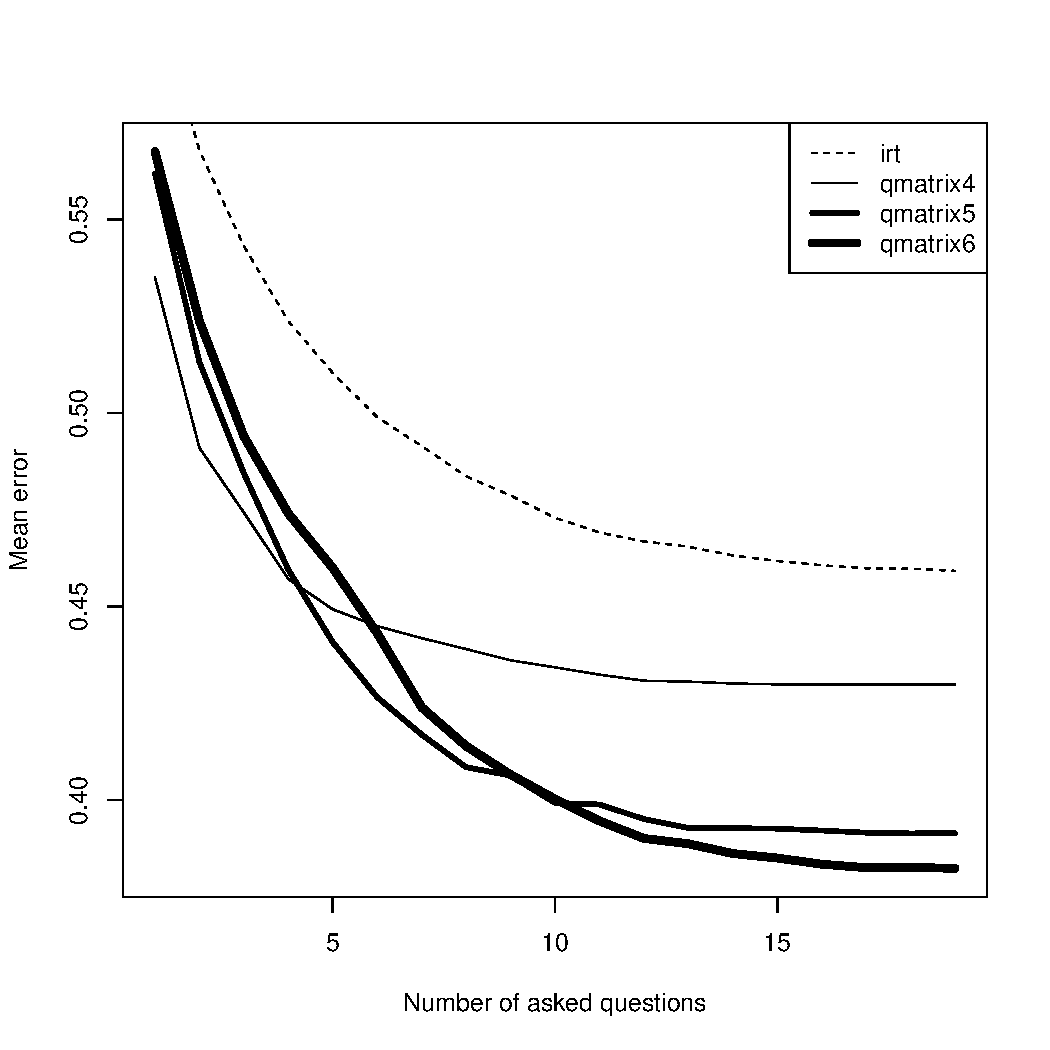
\includegraphics[width=\linewidth]{20-80.pdf}
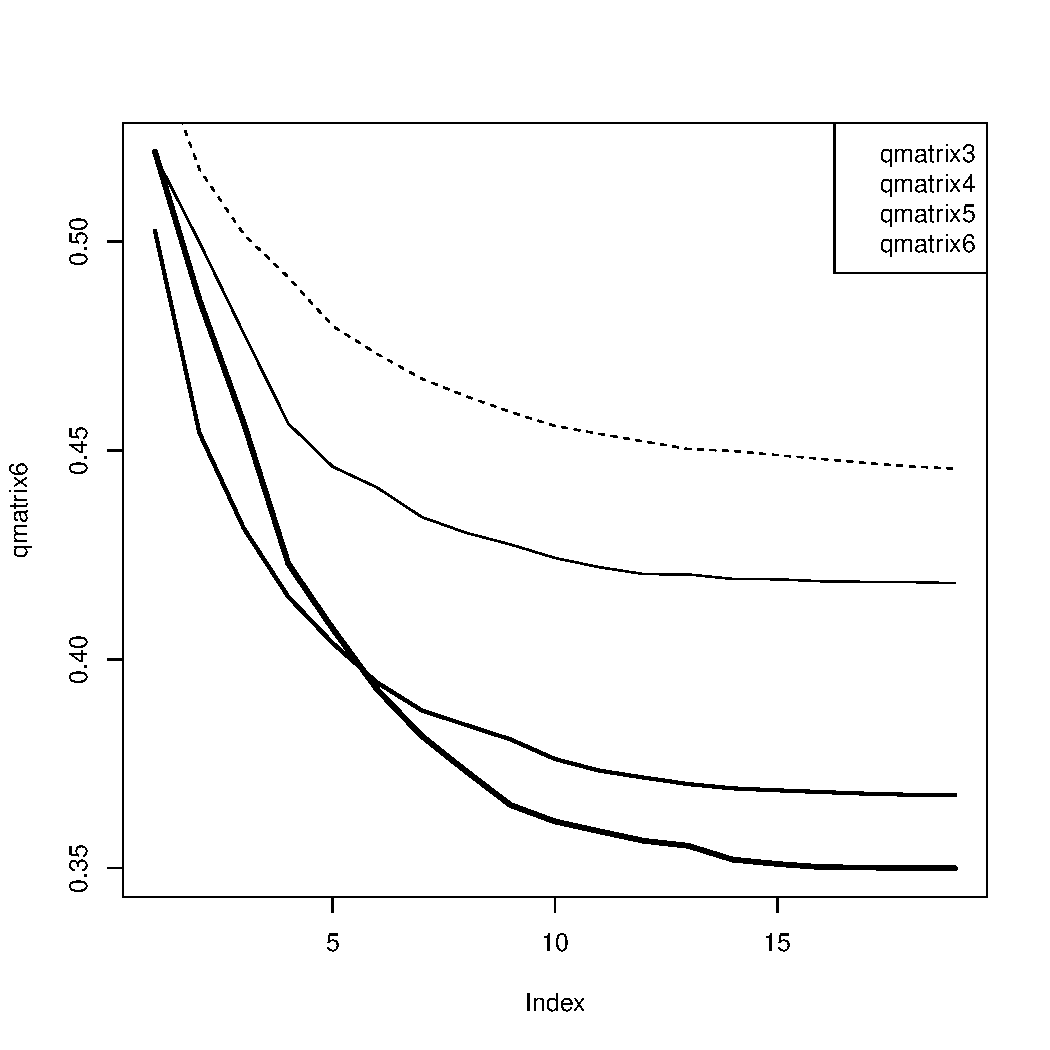
\includegraphics[width=\linewidth]{20-160.pdf}
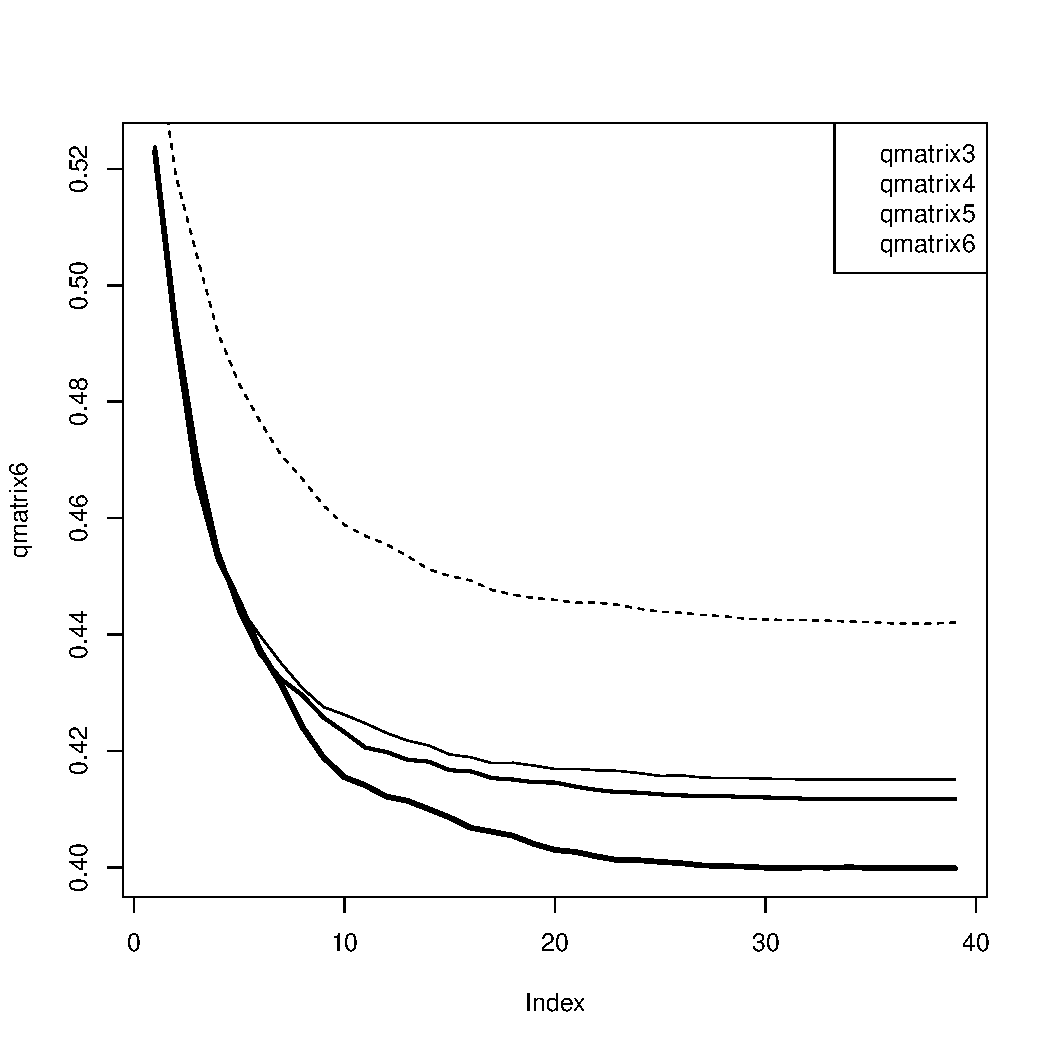
\includegraphics[width=\linewidth]{40-160.pdf}

\section{Discussion and Future Work}
Results are produce from one relatively small dataset. Interesting to try with other student datas (only one domain student dataset, bigger student dataset, ...). 

Interesting to study the K optimal depending on the number of students in the training set and the number of questions. There is a tradeoff to solve between big K potentially leading to over fitting and smaller ones which could not provide a rich enough model. Our results suggest that q-matrix is not very sensitive to the choice of K as long as this K parameters keep being reasonable given the train dataset. 

The results show that the interdependencies between question is important enough to be worth taking into account, the main difference between IRT and q-matrix being the fact that q-matrix capture these interdependencies. Other models taking into accounts these interdependence exists such as fusion models [explain]. We wouldn't be surprise if these kind of fusion model perform better than the NIDA q-matrix model presented here. 

One important aspect is the training step. It appear that our implementation of q-matrix was limited by the approximation of the q-matrix done during the training step and amelioration can be done in this direction, particularly for bigger q-matrix ($K \ge 6$). 


%Add a last column to q-matrix

%No study has been done yet over the number of skills.

%Outperforms on both simulated data and real data.

%\section{Acknowledgments}

% The following two commands are all you need in the
% initial runs of your .tex file to
% produce the bibliography for the citations in your paper.
%\bibliographystyle{abbrv}
\bibliographystyle{plainnat}
\bibliography{sigproc}  % sigproc.bib is the name of the Bibliography in this case
% You must have a proper ".bib" file
%  and remember to run:
% latex bibtex latex latex
% to resolve all references
%
% ACM needs 'a single self-contained file'!
%
%APPENDICES are optional
%\balancecolumns
%\appendix
%Appendix A
%\section{If I have something more to say}

%\balancecolumns % GM June 2007
% That's all folks!
\end{document}
